\documentclass[11pt, english]{article}
\usepackage[svgnames]{xcolor}
\usepackage{booktabs}
\usepackage{graphicx}
\usepackage[flushleft]{threeparttable}
\usepackage[colorlinks=true, linkcolor=blue]{hyperref}
\usepackage{float}
\usepackage[utf8]{inputenc}
\usepackage[T1]{fontenc}
\usepackage[utf8]{inputenc}
\usepackage{listingsutf8}
\usepackage[spanish]{babel}
\selectlanguage{spanish}
\usepackage{amsmath}


\usepackage{listings}
\usepackage{afterpage}

\pagestyle{plain}

\definecolor{dkgreen}{rgb}{0,0.6,0}
\definecolor{gray}{rgb}{0.5,0.5,0.5}
\definecolor{mauve}{rgb}{0.58,0,0.82}
%\lstset{language=R,
%    basicstyle=\small\ttfamily,
%   stringstyle=\color{DarkGreen},
%    otherkeywords={0,1,2,3,4,5,6,7,8,9},
%    morekeywords={TRUE,FALSE},
%    deletekeywords={data,frame,length,as,character},
%    keywordstyle=\color{blue},
%    commentstyle=\color{DarkGreen},
%}

\lstset{frame=tb,
	language=Java,
	aboveskip=3mm,
	belowskip=3mm,
	showstringspaces=false,
	columns=flexible,
	numbers=none,
	keywordstyle=\color{blue},
	numberstyle=\tiny\color{gray},
	commentstyle=\color{dkgreen},
	stringstyle=\color{mauve},
	breaklines=true,
	breakatwhitespace=true,
	tabsize=3,
	inputencoding=utf8/latin1,
	extendedchars=true,
	literate={á}{{\'a}}1 {é}{{\'e}}1 {ó}{{\'o}}1 {ú}{{\'u}}1 {ü}{{\"u}}1 {ñ}{{\~n}}1 {¿}{{?`}}1 {¡}{{!`}}1
}

\usepackage{here}


\textheight=21cm
\textwidth=17cm
%\topmargin=-1cm
\oddsidemargin=0cm
\parindent=0mm
\pagestyle{plain}

%%%%%%%%%%%%%%%%%%%%%%%%%%
% La siguiente instrucción pone el curso automáticamente%
%%%%%%%%%%%%%%%%%%%%%%%%%%

\usepackage{color}
\usepackage{ragged2e}

\global\let\date\relax
\newcounter{unomenos}
\setcounter{unomenos}{\number\year}
\addtocounter{unomenos}{-1}
\stepcounter{unomenos}
\gdef\@date{ Curso  2018 / \arabic{unomenos}}

\begin{document}
	
	\begin{titlepage}
		
		\begin{center}
			\vspace*{-1in}
			\begin{figure}[htb]
				\begin{center}
					\includegraphics[width=10cm]{../res/pics/logo.jpg}
				\end{center}
			\end{figure}
			
			\vspace*{0.4in}
			\begin{large}
				\textsc{Procesadores de Lenguaje}:\\
			\end{large}
			\vspace*{0.2in}
			\begin{Large}
				\textbf{\textsc{WiC}}\\
			\end{Large}
			\vspace*{0.3in}
			\begin{large}
				\@date\\
			\end{large}
			\vspace*{0.3in}invalid utf-8 byte sequence spanish characters listing latex
			\rule{80mm}{0.1mm}\\
			\vspace*{0.1in}
			\begin{large}
				Realizado por: \\
				
				Medina Medina, David Alberto  \\
				Brito Ramos, Christian  \\
				Hernández Delgado, Christopher \\
				López González, Néstor \\
				\vspace*{0.3in}
			\end{large}
			
\includegraphics[width=3cm]{../res/pics/LogoEscuela.jpg}
		\end{center}
	\end{titlepage}
	
	\newcommand{\CC}{C\nolinebreak\hspace{-.05em}\raisebox{.4ex}{\tiny\bf +}\nolinebreak\hspace{-.10em}\raisebox{.4ex}{\tiny\bf +}}
	\def\CC{{C\nolinebreak[4]\hspace{-.05em}\raisebox{.4ex}{\tiny\bf ++}}}
	
	\tableofcontents
	\newpage
	
	\abstract{
		\texttt{WiC} (Winter is Coming) es un lenguaje de programación diseñado por estudiantes de la \textit{ULPGC} con el objetivo de establecer el diseño y desarrollo de un compilador de lenguaje. El objetivo de esta experiencia es desarrollar un compilador del lenguaje que pase por las diferentes etapas de análisis léxico, sintáctico y semántico con el objetivo de generar un código intermedio en lenguaje ensamblador \texttt{IA-32}}\label{Resumen}
	
	\section{Definición del lenguaje}\label{Definicion-lenguaje}
	En esta sección se describen todos los detalles que describen las características propias del lenguaje \texttt{WiC}.
	
	\subsection{Tipos de datos}\label{data-type}
	Cualquier leguaje de programación necesita definir un conjunto de \emph{tipos de datos}, esto es, la batería de valores y operaciones que puede adquirir una variable. Cada tipo de dato está definido en el lenguaje por un \emph{literal} único que lo representa, lo que permite que cada tipo de dato tenga un representación física específica.
	
	Los tipos de datos definidos en el lenguaje son los que figuran en el \emph{cuadro \ref{tab:table1}}. Las características críticas de implementación que define a cada tipo son:
	
	\begin{description}
		\item[Entero] Representa a todas y cada una de las variables enteras que sean declaradas en el lenguaje. Este tipo de dato presenta un tamaño de 4 bytes (32 bits) y permite representar números enteros con signo. El \emph{complemento a 2} es el sistema elegido para definir el signo del número entero. Este dato se representa por el literal \texttt{int}. El rango de valores que puede tomar es
		
		\begin{equation}\label{eq:equation1}
		\left [-2^{N-1},\: 2^{N-1}-1 \right ] = \left [-2^{32-1},\: 2^{32-1}-1 \right] = \left [-2147483648,\: 2147483647 \right]
		\end{equation}
		
		donde, $N$ es el número de bits disponibles para representar el número entero (32 bits).
		\item[Coma flotante de simple precisión] Este tipo de dato representa número reales en coma flotante de simple precisión con un tamaño de 4 bytes (32 bits) siguiendo el estándar \emph{IEEE 754}. En la figura \ref{fig:figure1} puede observarse como esta representación binaria los bits se organizan en tres sectores principales:
		\begin{itemize}
			\item \textbf{Signo} (1 bit). Se trata de un sólo bit que define el signo del número: positivo (0) o negativo (1).
			\item  \textbf{Exponente (8bits)}. Se trata de un número entero con signo de complemento a 2 ($\left [ -128,\: 127\right ]$)
			\item \textbf{Mantisa (23 bits)}. Conforma la fracción a la derecha de la coma binaria y un bit de encabezado implícito.
		\end{itemize}
		Este tipo de dato se representa con el literal \texttt{real}. Su rango de valores es de $\left [ 1.18 \cdot 10^{–38},\; 3.4 \cdot 10^{38} \right ]$.
		\begin{figure}[H]\label{fig:figure1}
			\centering
			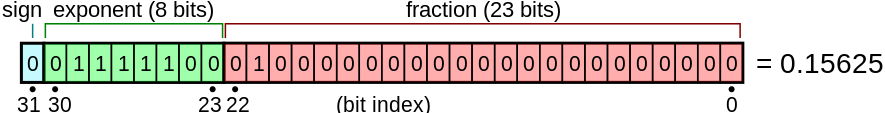
\includegraphics[width=0.75\textwidth]{../res/pics/data-types/float_diag.png}
			\caption{Representación binaria de número en coma flotante de simple precisión (\emph{IEEE 754})}
		\end{figure}
		
		\item[Caracter] Este tipo de dato es usado para representar caracteres con la codificación \emph{ASCII}, es por este motivo que el tamaño de que ocupan las variables de tipo caracter son de 1 byte de tamaño, siendo \texttt{char} el literal que lo representa.
		\item[Booleano] Se trata de un tipo de dato utilizado para representar representar valores booleanos. Su tamaño es de 1 bit, por lo que tan solo puede tomar dos valores: \texttt{1} (verdadero) ó \texttt{0} (falso). El literal que lo representa es \texttt{bool}.
	\end{description}
	
	\begin{table}[H]
		\begin{center}
			\caption{Tipos de datos}
			\label{tab:table1}
			\begin{tabular}{l|l|l|l}
				\toprule
				\textbf{Tipo} & \textbf{Literal} & \textbf{Tamaño} & \textbf{Rango}\\
				\midrule
				Entero & int & 4 Bytes & $\left [-2147483648,\: 2147483647 \right]$\\
				Coma flotante de simple precisión & real & 4 Byte & $\left [ 1.18 \cdot 10^{–38},\; 3.4 \cdot 10^{38} \right ]$\\
				Caracter & char & 1 Byte & $\left [ \texttt{0x00 - 0xFF} \right ]$\\
				Lógico & bool & 1 Bit & $\left [0,\; 1 \right ]$\\
				\bottomrule
			\end{tabular}
		\end{center}
	\end{table}
	
	En el siguiente ejemplo se muestra cómo se declaran las variables con los literales de los tipos descritos anteriormente:
	
	\lstinputlisting[language=C++]{../res/lst/data-types/data-type.x}
	
	\subsection{Colecciones de datos: \texttt{Arrays}}\label{arrays}
	Las variables pueden ser agrupadas en colecciones de datos de una dimensión denominados \texttt{arrays}. En este lenguaje, cualquier tipo de dato puede formar parte de un \texttt{array}.
	
	Para declarar un \texttt{array} del tipo que se desee, debe usar la gramática \ref{grammar:1.2.1}:
	\begin{equation}\label{grammar:1.2.1}
	tipo[<int>]\; nombre\_variable
	\end{equation}
	
	donde el $tipo$ define el tipo de dato e $<int>$ un valor entero opcional que define el tamaño del \texttt{array}. Cuando no se indica este último valor entero, no se lleva a término la reserva en memoria del \texttt{array} declarado. En caso contrario, se reservará en memoria tantos bytes/bits como fueren necesarios para generar una colección de tipos de datos del tamaño indicado por $<int>$. El número de bytes/bits a reservar está determinado por el tipo de dato y el tamaño del \texttt{array},
	\begin{equation}\label{eq:1.2}
	Tamano_{memoria} = Tamano_{tipo\, dato} \times Tamano_{array}
	\end{equation}
	
	Un \texttt{array} que ha sido declarado con anterioridad puede ser redefinido haciendo uso de la gramática \ref{grammar:1.2.2},
	\begin{equation}\label{grammar:1.2.2}
	tipo[ \, ]\; nombre\_variable = new\; tipo[<int>]\; \{ \\
	expresion\_1, expresion\_2, ...\;\}
	\end{equation}
	
	Esta notación es alternativa a la gramática \ref{grammar:1.2.1}, donde podremos inicializar el \texttt{array} a un conjunto de expresiones separados por comas encerrados dentro de los caracteres \texttt{\{} y \texttt{\}}. Estas expresiones son opcionales. El tamaño máximo del vector y, por tanto, de expresiones es el indicado por $<int>$ el cual es un número entero de caracter obligatorio.
	
	Si se declara un \texttt{array} utilizando la gramática \ref{grammar:1.2.1} o \ref{grammar:1.2.2} sin expresiones en esta última, el array es inicializado en todas sus posiciones al valor \texttt{0} para tipos de datos enteros y reales. Para caracteres el valor por defecto es el caracter \texttt{nulo}. Y para tipos booleanos el valor por defecto es \texttt{FALSE}.
	
	La gramática \ref{grammar:1.2.3} es necesaria para acceder al valor de un elemento del \texttt{array} en una posición arbitraria del mismo,
	\begin{equation}\label{grammar:1.2.3}
	nombre\_variable\; [<int>]
	\end{equation}
	donde $<int>$ es un entero obligatorio que indica la posición del \texttt{array} a la que se desea acceder.
	
	El \texttt{array} de caracteres constituyen los denominados \texttt{string}, los cuales requieren una atención especial ya que es posible cargar una variable con una secuencia de caracteres sin ser necesaria la declaración dada por la gramática \ref{grammar:1.2.2}. La gramática \ref{grammar:1.2.4} define la instancia de un \texttt{string} con un conjunto de caracteres localizados entre los caracteres comillas doble,
	
	\begin{equation}\label{grammar:1.2.4}
	nombre\_variable\; = " <char><char>..."
	\end{equation}
	
	El siguiente listado muestra algunos ejemplos de uso de los \texttt{array} definidos en este lenguaje:
	
	\lstinputlisting[language=C++, caption=Ejemplo de uso de arrays]{../res/lst/array/array.x}
	
	\subsection{Palabras reservadas y cambios de contexto}
	Este lenguaje utiliza una serie de palabras reservadas que se utilizan para desempeñar las funciones aquí descritas:
	\begin{description}
		\item[\texttt{continue}] La sentencia de continue es de tipo de control de bucles. Dentro de la iteracion en un bucle, de cualquiera de los tipos (while, do-while, for), el uso de esta sentencia rompe la iteracion de dicho bucle. Provocando que se ejecute la siguiente iteracion de dicho bucle, ignorando las sentencias posteriores a "continue".
		\item[\texttt{break}] Dentro de la iteracion en un bucle, de cualquiera de los tipos (while, do-while, for), el uso de esta sentencia rompe la iteracion de dicho bucle.
		\item[\texttt{return}] Palabra empleada para retornar el resultado de un método o función, además de interrumpir la ejecución del mismo.
		\item[\texttt{void}] Es utilizado para indicar que una función no debe devolver ningún valor.
		\item[\texttt{fun}] Palabra especial utilizada al principio de cada declaración o definición de funciones.
	\end{description}
	
	Los \textbf{cambios de contexto} de bloques de instrucciones son aplicables cuando se hace uso de un caracter \texttt{0x09} (\texttt{TAB}) o de 4 espacios consecutivos (\texttt{0x20}).
	
	\subsection{Comentarios}
	Aquí va el texto. Poner siempre un código de ejemplo.
	\begin{itemize}
		\item \textbf{'Comentario de línea'} . Para indicar un comentario de línea, basta con comenzar con '..', siendo el resultado final '.. {TEXTO}'.
		\begin{lstlisting}[caption=Ejemplo de comentario de línea]
		int a = 7
		.. Variable que almacena una suma.
		int suma = 0
		suma = 30 + a
		\end{lstlisting}
		\item \textbf{'Comentario de bloque'} . Los comentarios de varias líneas se establecen utilizando ',.' y '.,'  quedando como resultado ',. {VARIAS LÍNEAS DE TEXTO} .,'.
		\begin{lstlisting}[caption=Ejemplo de comentario de bloque]
		int a = 7
		int suma = 0
		suma = 30 + a
		,.
		En este punto, la variable suma toma el
		valor de 37.
		.,
		\end{lstlisting}
	\end{itemize}
	
	\subsection{Tipos de operadores}\label{operators}
	El conjunto de posibles operadores aplicables a nuestro lenguaje pueden clasificarse en:
	\begin{itemize}
		\item Operadores aritméticos
		\item Operadores lógicos
		\item Operadores bit a bit
		\item Operadores de array
	\end{itemize}
	
	
	\subsubsection{Operadores aritméticos}\label{arithmetic-operators}
	Estos operadores son necesarios para realizar operaciones matemáticas sencillas. La descripción detallada de cada uno de estos operadores queda reflejado en la tabla \ref{tab:arithmetic}.
	
	\begin{table}[H]
		\begin{center}
			\caption{Operadores aritméticos}\label{tab:arithmetic}
			\begin{threeparttable}
				\begin{tabular}{l|l|l|l|l|l}
					\toprule
					\textbf{Operación} & \textbf{Tipo operación} & \textbf{Lexema} & \textbf{Estructura} & \textbf{Tipo expresión} & \textbf{Tipo evaluado} \tnote{1}\\
					\midrule
					Suma  & Binaria & \texttt{+} & \texttt{\{Expr\} + \{Expr\}} & \texttt{int/real} & \texttt{int/real}\\
					Resta & Binaria & \texttt{-} & \texttt{\{Expr\} - \{Expr\}} & \texttt{int/real} & \texttt{int/real}\\
					Multiplicación & Binaria & \texttt{*} & \texttt{\{Expr\} * \{Expr\}} & \texttt{int/real} & \texttt{int/real}\\
					División & Binaria & \texttt{/} & \texttt{\{Expr\} / \{Expr\}} & \texttt{int/real} & \texttt{int/real}\\
					Módulo & Binaria & \texttt{\%} & \texttt{\{Expr\}\, \% \{Expr\}} & \texttt{int/real} & \texttt{int/real}\\
					Potencia & Binaria & \texttt{**} & \texttt{\{Expr\} ** \{Expr\}} & \texttt{int/real} & \texttt{int/real}\\
					Raíz & Binaria & \texttt{\#} & \texttt{\{Expr\} \# \{Expr\}} & \texttt{int/real} & \texttt{int/real}\\
					Pre-incremento \tnote{2} & Unaria & \texttt{++} & ++\texttt{\{Expr\}} & \texttt{int/real} & \texttt{int/real}\\
					Pre-decremento \tnote{2} & Unaria & \texttt{$--$} & $--$\texttt{\{Expr\}} & \texttt{int/real} & \texttt{int/real}\\
					Post-incremento \tnote{3} & Unaria & \texttt{++} & \texttt{\{Expr\}++} & \texttt{int/real} & \texttt{int/real}\\
					Post-decremento \tnote{3} & Unaria & \texttt{$--$} & \texttt{\{Expr\}$--$} & \texttt{int/real} & \texttt{int/real}\\
					\bottomrule
				\end{tabular}
				\begin{tablenotes}
					\small
					\item[1] Todas las operaciones binarias permiten entremezclar el uso de un valor entero y otro real al mismo tiempo aunque esto conllevaría el \textit{casteo} del resultado de la operación a un valor de tipo real.
					\item [2] El valor de la variable es incrementado/decrementado una unidad previa asignación del mismo.
					\item[3] El valor de la variable es incrementada/decrementada una unidad después de asignar el valor del misma.
				\end{tablenotes}
			\end{threeparttable}
		\end{center}
	\end{table}
	
	\begin{lstlisting}[caption=Ejemplo de uso los operadores artiméticos]
	int a = 2
	int b = 4
	
	int c = 2#4			..c = 2
	
	int d
	d = c++				..d = 2, c = 3
	
	int e
	e = ++c				..e = 4, c = 4
	\end{lstlisting}
	
	\subsubsection{Operadores lógicos}
	Definimos los símbolos que identificarán a los operadores lógicos de forma análoga a los utilizados por gran parte de otros lenguajes de programación, separando cada operador 2 expresiones a comparar por los operadores lógicos a utilizar, con la excepción del propio \emph{NOT}, que podrá utilizarse directamente para determinar si el valor devuelto por una expresión de tipo \texttt{booleano} es directamente verdadero o no. 
	
	% Esto puede que no de tiempo de implementarlo
	
	Como dato adicional, también consideramos la posibilidad de hacer uso de comparadores mediante dichos operadores lógicos n-arios, comparando pares de expresiones entre sí de forma sucesiva siguiendo el orden de lectura de izquierda a derecha (que a efectos prácticos es lo mismo que hacer sucesivos \emph{AND} pero de forma más breve) y la posibilidad de prioridades para ciertos operadores (como el \emph{AND}). \vspace{0px}
	
	En relación a las expresiones de comparación, consideramos hacer que de momento solo se puedan utilizar entre tipos de datos del mismo tipo o similar (por ejemplo, entre enteros y reales podría hacerse). Dejamos la tabla de operadores como sigue: \vspace{0px}
	
	\begin{table}[H]
		\begin{center}
			\caption{Operadores lógicos}\label{tab:logic-operators}
			\begin{threeparttable}
				\begin{tabular}{l|lllll}
					\toprule
					\textbf{Operación} & \textbf{Tipo operación} & \textbf{Lexema} & \textbf{Estructura} & \textbf{Tipo expresión}\tnote{1} & \textbf{Tipo evaluado}\\
					\midrule
					\texttt{AND} & Binaria & \texttt{\&\&} & \texttt{\{Expr\} \&\& \{Expr\}} & \texttt{int/real/bool} & \texttt{bool}\\
					\texttt{OR} & Binaria & \texttt{||} & \texttt{\{Expr\} || \{Expr\}} & \texttt{int/real/bool} & \texttt{bool}\\
					\texttt{NOT} & Unaria & \texttt{!} & \texttt{!\{Expr\}} & bool & \texttt{bool}\\
					Igual & Binaria & \texttt{==} & \texttt{\{Expr\} == \{Expr\}} & \texttt{int/real/bool} & \texttt{bool}\\
					No Igual & Binaria & \texttt{!=} & \texttt{\{Expr\} != \{Expr\}} & \texttt{int/real/bool} & \texttt{bool}\\
					Mayor & Binaria & \texttt{>} & \texttt{\{Expr\} > \{Expr\}} & \texttt{int/real/bool} & \texttt{bool}\\
					Mayor o igual & Binaria & \texttt{>=} & \texttt{\{Expr\} >= \{Expr\}} & \texttt{int/real/bool} & \texttt{bool}\\
					Menor & Binaria & \texttt{<} & \texttt{\{Expr\} < \{Expr\}} & \texttt{int/real/bool} & \texttt{bool}\\
					Menor o igual & Binaria & \texttt{<=} & \texttt{\{Expr\} <= \{Expr\}} & \texttt{int/real/bool} & \texttt{bool}\\
					\bottomrule
				\end{tabular}
				\begin{tablenotes}
					\small
					\item[1] El tipo de dato utilizado como expresión deben ser del mismo tipo para operadores lógicos binarios.
				\end{tablenotes}
			\end{threeparttable}
		\end{center}
	\end{table}
	
	\begin{lstlisting}[caption=Ejemplo de uso los operadores lógicos]
	int a = 7
	int suma = 0
	5 <= a < 10 ?:
	suma = 4 * a
	
	suma > 20 > a && 2*suma  < a
	suma++
	\end{lstlisting}
	
	\subsubsection{Operadores bit a bit}\label{bitwise-operators}
	Estos operadores permiten manipular los valores de una expresión a nivel de bits. El cuadro \ref{tab:bitwise} refleja la descripción detallada de cada uno de estos operadores.
	
	\begin{table}[H]
		\begin{center}
			\caption{Operadores bit a bit}\label{tab:bitwise}
			\begin{threeparttable}
				\begin{tabular}{l|l|l|l|l|l}
					\toprule
					\textbf{Operación} & \textbf{Tipo operación} & \textbf{Lexema} & \textbf{Estructura} & \textbf{Tipo expresión}\tnote{1} & \textbf{Tipo evaluado}\tnote{2}\\
					\midrule
					\texttt{AND} & Binaria & \texttt{\&} &  \texttt{\{Expr\} \& \{Expr\}} & Cualquiera & Cualquiera\\
					\texttt{OR} & Binaria & \texttt{|} &  \texttt{\{Expr\} | \{Expr\}} & Cualquiera & Cualquiera\\
					\texttt{XOR} & Binaria & \texttt{\textasciicircum} &  \texttt{\{Expr\} \textasciicircum \, \{Expr\}} & Cualquiera & Cualquiera\\
					Desp. izq. & Unaria & \texttt{\textless\textless} &  \texttt{\{Expr\} \textless\textless\, \{Expr\}}\tnote{3}\,& Cualquiera & Cualquiera\\
					Desp. dcha. & Unaria & \texttt{\textgreater\textgreater} & \texttt{\{Expr\} \textgreater\textgreater\, \{Expr\}}\tnote{3}\, & Cualquiera & Cualquiera\\
					\bottomrule
				\end{tabular}
				\begin{tablenotes}
					\small
					\item[1] El segundo operando debe ser siempre de tipo \texttt{int}.
					\item[2] El tipo de dato asignado a la variable debe ser del mismo tipo que el del primer operando.
					\item[3] Rota los bits de la expresión de la izquierda tantas unidades a la izquierda/derecha como indique la expresión de la derecha.
				\end{tablenotes}
			\end{threeparttable}
		\end{center}
	\end{table}
	
	\begin{lstlisting}[caption=Ejemplo de uso los operadores bit a bit]
	char c = ' '			.. c ==> Caracter ASCII 0x20
	int i = 2
	
	char rc = c<<2			.. rc = '@' ==> Caracter ASCII 0x40
	int ri = i<<2  		.. ri = 8
	
	\end{lstlisting}
	
	\subsubsection{Operadores de array}
	Los operadores de arrays nos permiten realizar operaciones con arrays, tratándolos como a subconjuntos. Los operadores a definir son los siguientes:
	\begin{description}
		\item [Unión] La unión de dos arrays consiste en crear un nuevo array formado por los elementos del primer array y los del segundo. La unión no permite elementos repetidos.
		\item [Diferencia] La  diferencia de un array con otro consiste en crear un nuevo array con todos los elementos del primer array, descartando aquellos que aparecen en el segundo.
		\item [Intersección] La intersección de dos arrays consiste en crear un nuevo array formado por todos los elementos comunes entre el primer y el segundo array.
		\item [Concatenación] Nuevo array formado por los elementos del primero seguido de los del segundo. La concatenación permite crear el nuevo array con elementos repetidos.
	\end{description}
	
	\begin{table}[H]
		\begin{center}
			\caption{Operadores de array}\label{tab:array-op}
			\begin{threeparttable}
				\begin{tabular}{l|l|l|l|l|l}
					\toprule
					\textbf{Operación} & \textbf{Tipo operación} & \textbf{Lexema} & \textbf{Estructura} & \textbf{Tipo expresión} & \textbf{Tipo evaluado}\\
					\midrule
					Unión & Binaria & \texttt{U} & \texttt{\{Expr\} U \{Expr\}} & Cualquiera & Cualquiera\\
					Diferencia & Binaria & \texttt{D} & \texttt{\{Expr\} D \{Expr\}} & Cualquiera & Cualquiera\\
					Intersección & Binaria & \texttt{I} & \texttt{\{Expr\} I \{Expr\}} & Cualquiera & Cualquiera\\
					Concatenación & Binaria & \texttt{+} & \texttt{\{Expr\} + \{Expr\}} & Cualquiera & Cualquiera\\
					\bottomrule
				\end{tabular}
				\begin{tablenotes}
					\small
					\item[1] Rota los bits de la expresión de la izquierda tantas unidades a la izquierda/derecha como indique la expresión de la derecha.
				\end{tablenotes}
			\end{threeparttable}
		\end{center}
	\end{table}
	
	A continuación mostramos un ejemplo de uso de los operadores de array para un caso trivial meramente ejemplificativo:
	\begin{lstlisting}[caption=Ejemplo de uso de operadores de array]
	int[6] a = {0,1,2,3,4,5}
	int[7] b = {3,4,5,6,7,8,9}
	
	int[] c = a U b 					..c = {0,1,2,3,4,5,6,7,8,9}
	int[] d = a D b 					..d = {0,1,2}
	int[] e = a I b 					..e = {3,4,5}
	int[] f = (a U b) D (a I b) 			..f = {0,1,2,6,7,8,9}
	int[] g = d + f + a 				..g = {0,1,2,0,1,2,6,7,8,9,0,1,2,3,4,5}
	\end{lstlisting}
	
	\subsection{Estructuras de control}
	El conjunto de instrucciones del lenguaje no tienen por qué ejecutarse en una secuencia lineal sino que es posible que el programador establezca un cierto control en esa secuencia de ejecución. Las diferentes estructuras de control que se definen en nuestro lenguaje se clasifican en los siguiente grupos:
	
	\begin{itemize}
		\item Sentencias \texttt{if-ifelse-else}
		\item Bucle \texttt{for-forelse-else}
		\item Bucle \texttt{while-whileelse-else}
	\end{itemize}
	
	\subsubsection{Sentencias \texttt{if-ifelse-else}}
	La estructura de control if-ifelse-else sentencia condicional que está compuesta de los siguientes bloques:
	\begin{description}
		\item[Bloque \texttt{if}] Este bloque está identificado por la siguiente estructura:
		\begin{center}
			\begin{lstlisting}
			{Expr} ?:
			{Instr}
			...
			\end{lstlisting}
		\end{center}
		En caso de ser verdadera, se ejecutan las instrucciones de este bloque. Sólo puede existir un único bloque \texttt{if} al principio de una sentencia \texttt{if-ifelse-else}.
		\item[Bloque \texttt{ifelse}] Si no se cumple la condición del bloque anterior, se comprueba si la condición de este bloque se cumple para posteriormente ejecutar el conjunto de instrucciones que se encuentran en su contexto. En caso contrario, pasa a ejecutarse el siguiente bloque \texttt{elseif} La estructura de este bloque es la siguiente:
		\begin{center}
			\begin{lstlisting}
			. {Expr} ?:
			{Instr}
			...
			\end{lstlisting}
		\end{center}
		\item[Bloque \texttt{else}] Si ninguna de la expresiones de los bloques anteriores cumple la condición, se ejecutarán las instrucciones contenidas en este bloque. La estructura de este bloque es la siguiente:
		\begin{center}
			\begin{lstlisting}
			.?:
			{Instr}
			...
			\end{lstlisting}
		\end{center}
		Sólo puede existir un único bloque \texttt{else} al final de una sentencia \texttt{if-ifelse-else}.
	\end{description}
	
	\begin{lstlisting}[caption=Ejemplo de uso de la sentencia \texttt{if-ifelse-else}]
	int a = 25
	int b = 0
	
	a > 20 ?:
	b = a - 10
	. a < 10 ?:
	b = a + 5
	.?:
	b = -1
	\end{lstlisting}
	
	\subsubsection{Bucle \texttt{for-forelse-else}}
	Este tipo de bucle permiten modificar el valor de una variable mientras se realiza la evaluación lógica de uno de sus bloques. El bucle for-forelse-else se estructura en los siguientes bloques:
	
	\begin{description}
		\item[Bloque \texttt{for}] Este bloque presenta la siguiente estructura:
		\begin{center}
			\begin{lstlisting}
			{Expr} ?? {Expr}:
			{Instr}
			...
			\end{lstlisting}
		\end{center}
		
		La primera expresión no exige que figure el parámetro utilizado en la iteración. Si, por ejemplo, se definen otras formas de salida dentro del contexto del bucle, y si se cumple la condición evaluada se ejecutarán las instrucciones dentro del contexto en caso de que el conjunto de condiciones del bucle se cumpla. Además, es legal no indicar una expresión lógica a evaluar, en cuyo caso, el resultado de la evaluación siempre será \texttt{true}, iterándose indefinidamente las instrucciones de este contexto. 
		
		La segunda expresión se usará comúnmente como modificador del valor de iteración empleado en la condición.
		
		\item[Bloque \texttt{forelse}] Se ha considerado hacer que exista el bloque \texttt{for-else}, que actuaría de tal manera que si no se cumple inicialmente la condición del primer bucle, comprobará la expresión del siguiente, y si su condición se cumple, estará evaluando repetidamente las instrucciones de este último (sin volver a comparar con las condiciones del bucle anterior al \texttt{else}). De esta manera, podemos hacer una estructura combinada de lo que en otros casos serían \texttt{if-for-else-for}, de forma directa con solo un \texttt{for-else}. \vspace{10px}Su estructura es la siguiente:
		\begin{center}
			\begin{lstlisting}
			. {Expr} ?? {Expr}:
			{Instr}
			...
			\end{lstlisting}
		\end{center}
		
		\item[Bloque \texttt{else}] De forma análoga a los \texttt{else} de las expresiones condicionales, la representación para este bloque es la siguiente:
		\begin{center}
			\begin{lstlisting}
			.??:
			{Instr}
			...
			\end{lstlisting}
		\end{center}
		
		Este bloque es siempre terminal al bucle \texttt{for-forelse-else} y siempre iterará por el conjunto de instrucciones de su contexto (bucle infinito) siempre y cuando las expresiones lógicas de los bloques anteriores evalúen a \texttt{false}.
	\end{description}
	\begin{lstlisting}[caption=Ejemplode uso del bucle for-forelse-else]
	int a = 7
	int b = 9
	int suma = 0
	int contador = 0
	
	a > contador ?? contador++:
	suma = suma + a * contador + b
	. b > contador ?? contador++:
	suma = suma + b*contador + a
	.??:
	suma = a + b
	.. Como 'a' es mayor que 'contador' inicialmente, solo se ejecutan instrucciones del primer bucle
	\end{lstlisting}
	
	\subsubsection{Bucle \texttt{while-whileelse-else}}\label{while}
	Este bucle permite ejecutar un bloque de instrucciones de manera iterativa siempre y cuando la condición de la expresión sea \texttt{true}. En caso contrario, se irá probando las diferentes condiciones de cada bloque del bucle. Este bucle se puede estructura en los siguientes bloques:
	
	\begin{description}
		\item[Bloque \texttt{while}] Este bloque está identificado por la siguiente estructura:
		\begin{center}
			\begin{lstlisting}
			{Expr} ??:
			{Instr}
			...
			\end{lstlisting}
		\end{center}
		Mientras la expresión del bloque siga sienda \texttt{true}, se ejecuta el bloque de instrucciones del bucle. Si la expresión es \texttt{false}, se evalúa la expresión lógica del siguiente bloque. Sólo puede existir un único bloque \texttt{while} al principio de un bucle \texttt{while-whileelse-else}.
		\item[Bloque \texttt{whileelse}] Si no se cumple la condición del bloque anterior, se comprueba si la expresión lógica de este bloque es \texttt{true}. Si es así, se itera por el conjunto de instrucciones que se encuentran en su contexto hasta que la expresión sea \texttt{false}. Si la evaluación de la expresión lógca es \texttt{false}, se pasa a ejecutar el siguiente bloque \texttt{whileelse} o el bloque terminal \texttt{else}. La estructura de este bloque es la siguiente:
		\begin{center}
			\begin{lstlisting}
			. {Expr} ??:
			{Instr}
			...
			\end{lstlisting}
		\end{center}
		\item[Bloque \texttt{else}] Si ninguna de la expresiones de los bloques anteriores cumple la condición, se iterarán las instrucciones contenidas en este bloque indefinidamente, generándose un bucle infinito termnial. La estructura de este bloque es la siguiente:
		\begin{center}
			\begin{lstlisting}
			.??:
			{Instr}
			...
			\end{lstlisting}
		\end{center}
		Sólo puede existir un único bloque \texttt{else} al final de un bucle \texttt{while-ifelse-else}.
	\end{description}
	
	En cualquier caso, la expresión lógica es opcional. Si no se indica una existe una expresión al principio del bucle, se itera por el conjunto de instrucciones de ese bloque de manera indefinida.
	
	
	\subsection{Declaración, definición y uso de funciones}\label{functions}
	Las funciones componen una estructura fundamental en cualquier lenguaje de programación que son útiles para estructurar funcionalmente el código en diferentes contextos, aportando una mayor expresividad del lenguaje.
	
	Una función puede ser declarada sin especificar el código que se ejecutará dentro de su contexto. La forma general de declaración puede observarse en el listado \ref{lst:fun-declaration}.
	
	\lstinputlisting[language=C++,caption=Declaración de funciones\label{lst:fun-declaration}]{../res/lst/function/function-declaration.x}
	
	La definición de cualquier función sigue la estructura del listado \ref{lst:fun-definition}. El cuerpo de la función debe comenzar por el caracter de cambio de contexto (caracter \texttt{0x09} o cuatro caracteres \texttt{0x20} seguidos).
	
	\lstinputlisting[language=C++,firstline=1,lastline=7, showlines=true, caption=Definición de funciones\label{lst:fun-definition}]{../res/lst/function/function-definition.x}
	
	El listado \ref{lst:fun-use} ilustra la estructura general de llamada a una función.
	
	\lstinputlisting[language=C++,firstline=1,lastline=7, showlines=true, caption=Declaracion de funciones\label{lst:fun-use}]{../res/lst/function/function-use.x}
	
	Es importante recalcar que la referencia en memoria de un array es leída cuando este es usado como parámetro de una función. Si un array es el valor de retorno de una función, se devuelve su referencia en memoria.
	
	
	\subsection{Funciones primitivas}
	En nuestro lenguaje, Van a existir predefinidas un conjunto de funciones primitivas que facilitarán al programador su trabajo en el desarrollo del programa. Las funciones están divididas en las siguientes categorías:
	
	\begin{description}
		\item [Interacción entrada-salida] Las funciones básicas de E/S son:
		\begin{description}
			
			\item[\texttt{bool print(T salida)}] Esta función permite mostrar por pantalla el valor de \texttt{salida}, cuyo tipo \texttt{T} puede ser \texttt{int, real, bool, char} o una string (\texttt{char[]}). Si la operación termina correctamente la primitiva devolverá \texttt{true}, en caso contrario, devuelve \texttt{false}.
			\item[\texttt{T scan(T entrada)}] Esta rutina permite leer el valor pasado por teclado una vez se pulse \texttt{ENTER} (\texttt{0x0D}). Si la operación termina satisfactoriamente la primitiva devolverá un valor de tipo  \texttt{T}, y en caso de que no se especifique, devuelve el valor en formato \texttt{string}.
			
			\begin{lstlisting}[caption=Ejemplo de uso de la función \texttt{print()} y \texttt{scan()}]
			int number
			char[] name
			print("Introduzca el primer número: ")
			a = scan()
			print("¿Cuál es su nombre? ")
			name = scan()
			print("El usuario " + name + " ha introducido el número " + number)
			\end{lstlisting}
		\end{description}
		
		% De aquí hacia abajo puede que no de tiempo de implementarlo
		
		\item [Funciones para arrays numéricos] Las funciones para arrays numéricos permiten operaciones que impliquen el uso de arrays. El tipo \texttt{T} de las siguientes funciones indica que el tipo del parámetro de entrada o el tipo de retorno de la función puede ser \texttt{int} ,  \texttt{real} ,  \texttt{bool} o \texttt{string}:
		
		\begin{description}
			\item [\texttt{int length(array)}] Devuelve el número de elementos del array.
			\item [\texttt{T[] delete(T[] array, int position)}] Elimina el elemento de la posición \texttt{position} del array y devuelve la referencia al array resultante. Los demás elementos a partir de la posición especificada serán desplazados una posición a la izquierda.
			\item [\texttt{bool equal(T[] array1, T[] array2)}] Devuelve \texttt{true} si los dos arrays son iguales en tamaño y los elementos están dispuestos en el mismo orden. En caso contrario, devuelve \texttt{false}.
		\end{description}
	\end{description}
	
	\begin{lstlisting}[caption=Ejemplo de uso de funciones primitivas para arrays numéricos]
	int[] v1 = {2,5,9,5}
	int[] v2 = {5,4,8,9,3}
	int tam = length(v1)			..tam = 4
	delete(v1,1)				..v1 = {5,9,5}
	boolean b1 = equal(v2,v1)		..b1 = false
	boolean b2 = equal(v1,v1)		..b2 = true
	\end{lstlisting}
	
	
	\subsection{Código ejemplo}\label{example-code}
	Por último, mostraremos varios ejemplos de programas en WiC con la finalidad de abarcar las subsecciones anteriores y tener una visión general de como funciona el lenguaje de programación.
	
	\vspace{5mm}
	El primer código de ejemplo consiste en mostrar por pantalla una suscesión de fibonacci que termina cuando un valor de la serie alcanza el valor de un dato introducido por teclado.
	
	\begin{lstlisting}[caption=Ejemplo de la función Fibonacci con parametros introducidos.]
	
	.. Variable global que contiene el resultado
	global int a = 0
	
	.. Funcion que actualiza los valores de a y b en funcion de sus valores anteriores
	fun void fibo()
	static int b = 1
	int aux = b
	b = a + b
	a = aux
	
	.. Leer de teclado un entero
	n = scan(int)
	
	.. Bucle que finaliza cuando a alcanza el valor introducido por teclado.
	( a < n ) ??:
	print(a)
	print(', ')
	fibo()
	print(crlf)
	
	\end{lstlisting}
	
	\begin{lstlisting}[caption=Salida en consola para '' n -> \  6 ''.]
	0, 1, 1, 2, 3, 5
	\end{lstlisting}
	\vspace{5mm}
	A continuación, mostramos el código de un programa que invierte el contenido de un array. Además, añadimos la condición de que en las posiciones impares, se sustituye el valor por un 0.
	
	\begin{lstlisting}[caption=Cambiar el orden de los elementos en un Array con condición.]
	
	..Inicializamos el vector que se va a invertir
	int [10] miVector = {0,1,2,3,4,5,6,7,8,9}
	
	.. Inicializamos el vector que contendrá el resultado, reservando el tamaño en memoria
	int [10] resultado
	
	.. Variable que contendrá el tamaño del vector a invertir
	int tamaño = length(miVector)
	
	.. Variable que emplearemos de contador para el bucle
	int contador = 0
	
	.. Recorremos las posiciones de los vectores
	contador <= tamaño ?? contador++:
	.. Si la posición actual es 'par'...
	contador\%2 == 0 ?:
	resultado [contador] = miVector[tamaño-contador-1]
	.. Si no es 'par'
	.?:
	miVector [contador] = 0
	
	., 
	Procedemos a imprimir el resultado con un bucle.
	Se precisa resetear el valor del contador.
	,.
	contador = 0
	print(''RESULTADO -> [ '')
	
	contador < tamaño-1 ?? contador++:
	print(resultado[contador])
	print('', '')
	
	print(resultado[tamaño-1])
	print('']'')
	
	
	\end{lstlisting}
	
	
	
	\section{Análisis léxico}\label{Definicion-lenguaje}
	En esta sección se describen todos los detalles que describen al analizador léxico del lenguaje \texttt{WiC}.
	
	\subsection{Introducción}\label{Introdución}
	El analizador léxico es la parte del compilador que se encarga de leer el flujo de caracteres que componen el programa fuente y agruparlos en tokens, que son agrupaciones de secuencias que guardan cierto significado; produciendo, para cada lexema, un token con la estructura $<nombre-token, valor-atributo>$. Cada token pasará a la fase del análisis sintáctico, a partir de la cuál se generará la gramática y el \textit{Árbol Sintáctico Abstracto} (\textit{AST}) asociado.
	
	
	En cada token, el primer componente (nombre-token) se utiliza para el análisis sintáctico, y el segundo (valor-atributo), el cual es opcional, apunta a una entrada de la tabla de símbolos con el valor de dicho token.
	
	\begin{lstlisting}[caption=Ejemplo de conversión de un conjunto de caracteres de un programa WiC en tokens]
	
	int doble = total * 2
	
	(int) 	-> 	INT_TYPE
	(doble) -> 	ID
	= 		-> 	ASSIGN
	(total) -> 	ID
	* 		-> 	PRODUCT
	2		->	INT_VAL
	
	\end{lstlisting}
	
	\subsection{Tabla de tokens}\label{Tabla de tokens}
	
	\begin{table}[H]
		\begin{tabular}{l|l|l|l}
			\toprule
			\textbf{Token} & \textbf{Valor-Atributo} & \textbf{Expresión-Regular}\\
			\midrule
			NEW & NO & $(new)$ \\
			CONTINUE & NO & $(continue)$ \\
			BREAK & NO & $(break)$ \\
			RETURN & NO & $(return)$ \\
			VOID & NO & $(void)$ \\
			FUN & NO & $(fun)$ \\
			GLOBAL & NO & $(global)$ \\
			STATIC	& NO & $(static)$ \\
			INT\_VAL & SI & $[0-9]+$ \\
			REAL\_VAL & SI & $([0-9]+\backslash.)[0-9]*|\backslash.[0-9]+$ \\
			BOOL\_VAR & SI & $(true|false)$ \\
			CHAR\_VAL & SI & <CHAR\_STATE>$[\textasciicircum']?|(\backslash \backslash[nrtvb'"])$ \\
			STRING\_VAL & SI & <STRING\_STATE>$[\textasciicircum"]|(\backslash\backslash[nrtvb'"])$ \\
			CHAR\_QUOTE & NO & <CHAR\_STATE>$\backslash '$ ó $\backslash '$ \\
			STRING\_QUOTE & NO & <STRING\_STATE>$\backslash "$ ó $\backslash "$ \\
			INT\_TYPE & NO & $(int)$ \\
			REAL\_TYPE  & NO & $(real)$ \\
			BOOL\_TYPE & NO & $(bool)$ \\
			CHAR\_TYPE & NO & $(char)$ \\
			IF\_CLAUSE & NO & $(\backslash?)\{1\}$ \\
			FOR\_WHILE\_CLAUSE & NO & $(\backslash?)\{2\}$ \\
			HEADER\_END & NO & $:$ \\
			ELSE\_IF\_FOR\_WHILE\_CLAUSE & NO & $(\backslash.)\{1\}$ \\
			OPEN\_CONTEXT\_TAG & NO & <CHECK\_LVL>$[\;]*$ \\
			CLOSE\_CONTEXT\_TAG & NO & <CHECK\_LVL>$[\;]*$ \\
			CLOSE\_CONTEXT\_TAG & NO & <CHECK\_LVL><<EOF>> \\
			ID & SI & $[a-zA-Z]([a-zA-Z]|[0-9])+$ \\
			ASSIGN & NO & $=$ \\
			SUM & NO & $\backslash+$ \\
			SUBSTRACT & NO & $-$ \\
			PRODUCT & NO & $\backslash*$ \\
			DIVIDE & NO & $/$ \\
			MODULUS & NO & $\%$ \\
			POWER & NO & $\backslash*\backslash*$ \\
			RADICAL & NO & $\#$ \\
			INCREMENT & NO & $++$ \\
			DECREMENT & NO & $--$ \\
			\bottomrule
		\end{tabular}
	\end{table}
	\begin{table}[H]
		\begin{tabular}{l|l|l}
			\toprule
			\textbf{Nombre-Token} & \textbf{Valor-Atributo} & \textbf{Expresión-Regular}\\
			\midrule
			AND\_BIT & NO & $\&$ \\
			OR\_BIT & NO & $|$  \\
			XOR\_BIT & NO & $\textasciicircum$ \\
			LEFT\_SHIFT & NO & $\textless\textless$ \\
			RIGHT\_SHIFT & NO & $\textgreater\textgreater$ \\
			AND & NO & $\&\&$ \\
			OR & NO & $||$ \\
			NOT & NO & $!$ \\
			EQUALS & NO & $==$ \\
			NOT\_EQUALS & NO & $!=$ \\
			GREATER & NO & $\textless$ \\
			GREATER\_EQUALS & NO & $\textgreater=$ \\
			LESS & NO & $\textless$ \\
			LESS\_EQUALS & NO & $\textless=$ \\
			UNION & NO & $U$ \\
			DIFFERENCE & NO & D \\
			INTERSECTION & NO & $I$ \\
			SQUARE\_BRACKET\_OPEN & NO & $\backslash [$ \\
			SQUARE\_BRACKET\_CLOSE & NO & $\backslash ]$ \\
			CURLY\_BRACKET\_OPEN & NO & $\backslash \{$ \\
			CURLY\_BRACKET\_CLOSE & NO & $\backslash \}$ \\
			ELEM\_SEPARATOR & NO & $,$ \\
			PARETHESES\_OPEN & NO & $\backslash($ \\
			PARETHESES\_CLOSE & NO & $\backslash)$ \\
			END\_OF\_INSTR & NO & $\backslash n$ \\
			\bottomrule
		\end{tabular}
	\end{table}
	
	\newpage
	
	\subsection{Estados}\label{Estados}
	
	El estado de un analizador léxico es la situación en la que se encuentra a la hora de interpretar los caracteres del programa fuente. Los estados posibles del analizador léxico son:
	
	\begin{description}
		\item[CHECK\_LVL] Este estado viene por defecto. En él, se comprueba el nivel en el que se encuentra el programa. Se llega a este estado al principio del programa o cuando se detecta un caracter de salto de línea. En todo estado de CHECK\_LVL, se comprueba el número de tabuladores (tomando el valor de un tabulador equivalente a cuatro espacios); con cada tabulador encontrado, se devuelve un token OPEN\_CONTEXT\_TAG si accedemos a un nivel estrictamente superior al que ya estábamos, y se devuelve CLOSE\_CONTEXT\_TAG si accedemos a un nivel estrictamente inferior al que ya estábamos. En caso de que ambos niveles sean exactamente iguales, no se devuelve ningún token, interpretando que no hay cambio de nivel.
		\item[INITIAL] En este estado, los caracteres son interpretados normalmente y se generan los tokens correspondientes.
		\item[COMMENT\_BLOCK] Este estado corresponde a los comentarios de bloque. Se llega a este estado cuando se detecta la expresión regular ",\.". A partir de este estado, todos los caracteres serán considerados como parte de un comentario y no se tendrán en cuenta en la generación de tokens. Cuando se detecta la expresión regular "\.,", se vuelve al estado INITIAL.
		\item[COMMENT\_LINE] Este estado corresponde a los comentarios de línea. Se llega a este estado cuando se detecta la expresión regular "\textbackslash{}.\textbackslash{}.". A partir de este estado, todos los caracteres serán considerados como parte de un comentario y no se tendrán en cuenta en la generación de tokens. Cuando se detecta , se vuelve al estado INITIAL.
		\item[CHAR\_STATE] Este estado corresponde a los caracteres. Se llega a este estado cuando se detecta el caracter comilla simple ("\'"). En este estado, solo es permitido que aparezca como máximo un caracter o dos si el primero es la barra invertida ('\'). Cuando se detecta otro caracter comilla simple, se vuelve al estado INITIAL.
		\item[STRING\_STATE] Este estado corresponde a las strings o cadenas de caracteres. Se llega a este estado cuando se detecta un caracter comillas dobles ("\""). A partir de este estado, todos los caracteres consecuentes formarán parte de una string. Cuando se detecta otro caracter comillas dobles, se vuelve al estado INITIAL.
	\end{description}
	
	\newpage
	
	\section{Análisis sintáctico}
	
	\subsection{El analizador sintáctico}
	
	El analizador sintáctico o parser constituye una representación intermedia del análisis de un programa. Su función es construir un árbol de análisis a partir de los componentes léxicos que recibe, aplicando las producciones de la gramática con el objetivo de comprobar la correctitud sintáctica del programa. Su salida es una representación de la cadena de componentes léxicos en forma de árbol sintáctico.
	\newline
	\newline
	Dicho de otro modo: el analizador sintáctico comprueba que el orden en que el analizador léxico le va entregando es válido, y para ello verifica que la cadena pueda ser generada por la gramática del lenguaje fuente.
	\newline
	\newline
	Otra de las funciones del analizador sintáctico es la de informar acerca de los errores en la sintaxis; recuperándose de los mismos, siempre que sea posible, para continuar procesando la entrada.
	
	\newpage
		
	Para comprobar si una cadena pertenece al lenguaje generado por una gramática, los analizadores sintácticos construyen una representación en forma de árbol de 2 posibles maneras:
	\newline
	\begin{description}
		\item[Analizadores sintácticos descendentes (Top-down)] Construyen el árbol sintáctico desde la raíz hasta las hojas, partiendo del símbolo inicial de la gramática (axioma) y expandiendo las producciones  hasta llegar a la cadena de entrada.
		\newline
		\item[Analizadores sintácticos ascendentes (Bottom-up)] Construyen el árbol sintáctico comenzando por las hojas, partiendo de los terminales de entrada y, mediante reducciones, llegan hasta el símbolo inicial. En este apartado, nos centraremos en los  analizadores  sintácticos ascendentes.
	\end{description}
	
	
	\subsection{Ejemplo de análisis sintáctico}
	
	Esta instrucción genera los siguientes tokens:
	
	\begin{lstlisting}
	
	int i = 0	-> INT_TYPE ID ASSIGN INT_VAL END_OF_INSTR
	
	\end{lstlisting}
	
	En este caso en concreto, se harán uso de las siguientes gramáticas:
	
	\begin{lstlisting}
	
	input 		:= instr END_OF_INSTR input | instr END_OF_INSTR
	instr 		:= data_init ID ASSIGN expr
	data_init 	:= data_type
	data_type	:= INT_TYPE
	expr 		:= INT_VAL
	
	\end{lstlisting}
	
	El analizador, cuando llega un token de entrada, puede hacer dos cosas:
	
	\begin{description}
		\item[] Si el token es una parte derecha de una regla (o completa una parte derecha en construcción), se puede  deshacer la regla. Esta acción es llamada reducción.\newline
		\newline\newline
		\item[] Si no se puede completar una parte derecha, se acumula a lo que se está construyendo. Esta acción es llamada desplazamiento.
	\end{description}

	En este caso, el analizador sintáctico realiza un análisis ascendente de la siguiente forma:
	
	\begin{description}
		
		\item[Cadena de entrada:] INT\_TYPE ID ASSIGN INT\_VAL END\_OF\_INSTR
		\item[Reducir data\_type := INT\_TYPE] data\_type ID ASSIGN INT\_VAL END\_OF\_INSTR
		\item[Reducir data\_init := data\_type] data\_init ID ASSIGN INT\_VAL END\_OF\_INSTR
		\item[Desplazar data\_init, ID, ASSIGN]
		\item[Reducir expr := INT\_VAL] data\_init ID ASSIGN expr END\_OF\_INSTR
		\item[Reducir instr := data\_init ID ASSIGN expr] instr END\_OF\_INSTR
		\item[Reducir input := instr END\_OF\_INSTR] input
		
	\end{description}
	
	\section{Descenso recursivo}
	
	\subsection{Introducción}
	
	El análisis sintáctico por descenso recursivo consiste en realizar un conjunto de procedimientos, uno para cada nodo no terminal. El algoritmo para un nodo terminal general tiene la siguiente estructura:
	
	\begin{lstlisting}
	
	void A () {
		elegir una producción A, A -> X1X2...Xk;
		for (i = 1 a k) {
			if (X es un nodo no terminal) {
				llamar al procedimiento Xi();
			} else if (X es igual al símbolo de entrada actual a) {
				avanzar la entrada hasta el siguiente símbolo;
			} else {
				/*No ha ocurrido ningún error*/
			}
		}
	}
	
	\end{lstlisting}
	
	Para volver recursivo este algoritmo, se elige más de una opción de producción. Para poder probar otra producción A, debemos establecer el apuntador de entrada a la posición inicial.
	
	\begin{lstlisting}
	
	void A () {
		elegir una producción A|B, A -> X1X2...Xk, B -> Y1Y2...Yk;
		for (i = 1 a k) {
			if (X es un nodo no terminal) {
				llamar al procedimiento Xi();
			} else if (X es igual al símbolo de entrada actual a) {
				avanzar la entrada hasta el siguiente símbolo;
			} else {
				return 1;
			}
		}
	}
	
	NOTA: el fallo del else (return 1) no sugiere que el análisis finaliza ahí.
	
	\end{lstlisting}
	
	\newpage
	
	
	
	\subsection{Ejemplo de análisis sintáctico por descenso recursivo}
	
	Esta instrucción genera los siguientes tokens:
	
	\begin{lstlisting}
	
	5 > i ?? i++:	-> INT_VAL, GREATER, ID, FOR_WHILE_CLAUSE, ID, INCREMENT, HEADER_END, END_OF_INSTR
	
	\end{lstlisting}
	
	En este caso en concreto, se harán uso de las siguientes gramáticas:
	
	\begin{lstlisting}
	
	input 		:= instr END_OF_INSTR input | instr END_OF_INSTR
	instr 		:= for_instr
	for_instr	:= expr FOR_WHILE_CLAUSE expr HEADER_END END_OF_INSTR input
	expr 		:= expr SUM term | ID INCREMENT | term
	term		:= INT_VAL
	
	\end{lstlisting}
	
	\newpage
	
	\section{Tabla de símbolos}
	
	\subsection{Introducción}
	
	La tabla de símbolos almacena la información que en cada momento se necesita sobre las variables del programa y otra información, como el nombre, el tipo, el tamaño... También sirve para guardar información referente a cualquier clase, enumerado, identificador, etc. creado por el usuario.
	\newline
	La gestión de la tabla de símbolos es muy importante, ya que consume gran parte del tiempo de compilación; de ahí que su eficiencia sea crítica.
	\newline
	Respecto a las variables de usuario, la información que puede ser almacenada en la tabla de símbolos se divide en:
	
	\begin{description}
		
		\item[Nombre] Se puede hacer con o sin límite. Si se hace con límite, emplearemos una longitud fija para cada variable, lo cual aumenta la velocidad de creación, pero limita la longitud en unos casos, y desperdicia espacio en la mayoría. Otro método es habilitar la memoria que necesitemos en cada caso para guardar el nombre.\newline
		\item[Tipo] Tipo de dato de la variable.\newline
		\item[Dirección de memoria] Esta dirección es necesaria, porque las instrucciones que referencian a una variable deben saber donde encontrar el valor de esa variable en tiempo de ejecución, también cuando se trata de variables globales.\newline
		\item[Número de dimensiones de una variable array, o el de parámetros de una función o procedimiento y tipo de cada uno de ellos] Puede ser útil para el chequeo semántico.\newline
		
	\end{description}
	
	La tabla de símbolos también resulta útil para almacenar información relativa a las constantes, palabras reservadas y funciones de librería.

	\newpage
	
	\subsection{Operaciones de la tabla de símbolos}

	La tabla de símbolos consta de una estructura llamada símbolo. Las operaciones que puede realizar son:
	
	\begin{description}
		
		\item[Crear] Crea una tabla vacía.\newline
		\item[Insertar] Añade un nodo a la cabeza de la tabla.\newline
		\item[Buscar] Busca el nodo que contiene el nombre pasado por parámetro.\newline
		\item[Imprimir] Devuelve una lista con los valores que tiene los identificadores de usuario, recorriendo la tabla de símbolos.\newline
		
	\end{description}

	\subsection{Ejemplo de uso de la tabla de símbolos}
	
	Suponemos que queremos hacer las siguientes operaciones:
	
		a = 7 * 3
		b = 3 * a
		a = a + b
	
	En la segunda instrucción necesitamos saber cuanto vale 'a'; es decir, el valor de 'a' debe estar guardado en algún sitio. Para ello utilizaremos una lista de pares nombre, valor; de forma que, cuando nos encontremos con la instrucción a = 7 * 3, miremos en la tabla y, si no está 'a' en la tabla, creamos un nodo para introducirla.
	\newline
	\begin{table}[H]
		\begin{center}
			\begin{tabular}{l|l}
				\toprule
				\textbf{Nombre} & \textbf{Valor}\\
				\midrule
				a	& 	21\\
				\bottomrule
			\end{tabular}
		\end{center}
	\end{table}
	\newline
	A continuación nos encontramos con b = 3 * a. Buscamos 'a' en la tabla de símbolos y vemos que el valor de 'a' es 21. Ahora buscamos 'b' en la tabla de símbolos y como no está lo creamos.
	\newline
	\begin{table}[H]
		\begin{center}
			\begin{tabular}{l|l}
				\toprule
				\textbf{Nombre} & \textbf{Valor}\\
				\midrule
				a	& 	21\\
				b	&	63\\
				\bottomrule
			\end{tabular}
		\end{center}
	\end{table}
	\newline
	Ejecutamos ahora la instrucción a = a + b. Tendríamos a 'a' y 'b' en la tabla de símbolos con lo cual solo tendríamos que modificar	el valor de 'a'.
	\newline
	\begin{table}[H]
		\begin{center}
			\begin{tabular}{l|l}
				\toprule
				\textbf{Nombre} & \textbf{Valor}\\
				\midrule
				a	& 	84\\
				b	&	63\\
				\bottomrule
			\end{tabular}
		\end{center}
	\end{table}
	\newline
	
\end{document}
